\documentclass{beamer}

\usepackage{focs-slides}
 \usepackage{tikz}
\usepackage{pifont}
\usepackage{xcolor}
\usepackage{amssymb}
\usepackage{pgf}
\usepackage{minted}
\usemintedstyle{perldoc}
\usepackage{lipsum} 
\usepackage{enumerate}
\usepackage{hyperref}

\usepackage[font=scriptsize,labelfont=bf]{caption}
\captionsetup{labelfont={color=black}}

\definecolor{aquamarineDark}{HTML}{013220}
\definecolor{aquamarineMid}{HTML}{45B39D}
\definecolor{aquamarineAccent}{HTML}{16A085}
\definecolor{aquamarineLight}{HTML}{A3E4D7}
\definecolor{aquamarineGrey}{HTML}{708090} 
\usetikzlibrary{arrows.meta}

\newcolumntype{C}[1]{>{\centering\arraybackslash}p{#1}}
\newcolumntype{L}[1]{>{\raggedright\arraybackslash}p{#1}}

\definecolor{bg}{rgb}{0.95,0.95,0.95}
\setminted{
    %bgcolor=black,
    linenos,
    breaklines,
    fontsize=\footnotesize,
    tabsize=4
}
\setmintedinline{
    fontsize=\footnotesize
}
\newcommand{\LC}[1]{\mintinline{latex}{ #1 }}
\newcommand{\LCL}[1]{\begin{minted}{latex}{
#1
}\end{minted}}
\usepackage[utf8]{inputenc}
\usepackage{tcolorbox}
\tcbuselibrary{minted,skins}

\definecolor{bill}{RGB}{0,0,0}
\definecolor{numC}{RGB}{220,220,220}

\newtcblisting{mycodepython}{
    listing engine=minted,
    minted style=perldoc,
    minted language=python,
    minted options={fontsize=\small,linenos,numbersep=3mm},
    %colback=bill,
    %colframe=bill,
    listing only,
    left=5mm,
    enhanced,
    overlay={\begin{tcbclipinterior}\fill[numC](frame.south west)rectangle([xshift=5mm]frame.north west);\end{tcbclipinterior}}
}

\newtcblisting{mycodejson}{
    listing engine=minted,
    minted style=perldoc,
    minted language=json,
    minted options={fontsize=\small,linenos,numbersep=3mm},
    %colback=bill,
    %colframe=bill,
    listing only,
    left=5mm,
    enhanced,
    overlay={\begin{tcbclipinterior}\fill[numC](frame.south west)rectangle([xshift=5mm]frame.north west);\end{tcbclipinterior}}
}

\newtcblisting{bashcode}{
    listing engine=minted,
    minted style=perldoc,
    minted language=bash,
    minted options={fontsize=\small,linenos,numbersep=3mm},
    %colback=bill,
    %colframe=bill,
    listing only,
    left=5mm,
    enhanced,
    overlay={\begin{tcbclipinterior}\fill[numC](frame.south west)rectangle([xshift=5mm]frame.north west);\end{tcbclipinterior}}
}

\newtcblisting{bashcodetiny}{
    listing engine=minted,
    minted style=perldoc,
    minted language=bash,
    minted options={fontsize=\scriptsize,linenos,numbersep=3mm},
    %colback=bill,
    %colframe=bill,
    listing only,
    left=5mm,
    enhanced,
    overlay={\begin{tcbclipinterior}\fill[numC](frame.south west)rectangle([xshift=5mm]frame.north west);\end{tcbclipinterior}}
}

\newtcblisting{mycodetiny}{
    listing engine=minted,
    minted style=perldoc,
    minted language=python,
    minted options={fontsize=\scriptsize,linenos,numbersep=2mm},
    %colback=bill,
    %colframe=bill,
    listing only,
    left=5mm,
    enhanced,
    overlay={\begin{tcbclipinterior}\fill[numC](frame.south west)rectangle([xshift=5mm]frame.north west);\end{tcbclipinterior}}
}

\newtcblisting{mycodesql}{
    listing engine=minted,
    minted style=perldoc,
    minted language=sql,
    minted options={fontsize=\footnotesize,linenos,numbersep=3mm},
    %colback=bill,
    %colframe=bill,
    listing only,
    left=5mm,
    enhanced,
    overlay={\begin{tcbclipinterior}\fill[numC](frame.south west)rectangle([xshift=5mm]frame.north west);\end{tcbclipinterior}}
}

\usepackage{forest}
\usetikzlibrary{
    shapes.geometric,  
    arrows.meta,        
    positioning,       
    fit,               
    backgrounds         
}
\usetikzlibrary{shapes.geometric, arrows.meta, positioning, fit, calc}
\tikzset{
    process/.style={
        draw, 
        rectangle, 
        rounded corners,
        fill=blue!15, 
        minimum height=3em, 
        text width=7em, 
        align=center
    },
    data/.style={
        draw, 
        rectangle, 
        fill=green!15,
        minimum height=3em,
        text width=6em, 
        align=center
    },
    io/.style={
        draw,
        trapezium,
        trapezium left angle=70, 
        trapezium right angle=110,
        fill=purple!15,
        minimum height=3em,
        text width=8em, 
        align=center
    },
    result/.style={
        draw,
        rectangle,
        fill=orange!20,
        text width=8em,
        align=center,
        minimum height=8em
    },
    annotation/.style={
        text width=10em, 
        align=left
    },
    container/.style={
        draw,
        dashed,
        inner sep=0.5cm,
        rounded corners
    },
    arrow/.style={
        -{{Stealth[length=3mm, width=2mm]}},
        thick
    }
}

\definecolor{aquamarineDark}{HTML}{254242}   % darker, close to primary but a bit teal-leaning
\definecolor{aquamarineMid}{HTML}{3E6C6C}    % mid tone, muted aquamarine that complements primary
\definecolor{aquamarineLight}{HTML}{A3CFCF}  % light background-ish tint for contrast
\definecolor{aquamarineGrey}{HTML}{6E7B7B}   % desaturated grey with same family
\definecolor{aquamarineAccent}{HTML}{1F5F5F} % deeper accent, richer than aquamarineDark for emphasis


\title{Drilling Into Sound}
\author{Team member names: Li Yanzhi, Zhang Lingwei, Zuo Tianyou, Aghamatlab Akbarzade}
\date{Summer 2025}
\course{ECE472}

% bibliography file
\addbibresource{project.bib}

\definecolor{darkblue}{HTML}{6666dd}
\definecolor{darkslategray}{HTML}{2f4f4f}
%\colortheme{green!42!black}
%\colortheme{orange!85!black}
%\colortheme{darkblue}
%\colortheme{pink!80!black}
%\colortheme{orange!85!white!90!black}
\colortheme{darkslategray}

\begin{document}

\maketitle

% table of contents
\toc{enum}
% \toc{mindmap}

\begin{section}{Overview}
    \begin{frame}{Introduction}
        We are a passionate team that aims to build a high-performance music platform based on the \textbf{Million Song Dataset}. To efficiently build our project, we divide our task into four milestones:
        
        \begin{enumerate}
            \item \textbf{M0: Data Extraction in Avro.} We perform proper feature engineering to get necessary song features from the original datasets and store them in avro format.
            \item \textbf{M1: Database Query with Drill.} We use Drill to query the datasets and validate our Avro files.
            \item \textbf{M2: Song Recommendation.} We give three different ideas to build our music platform into a diverse and customizable system.
            \item \textbf{M3: Year Prediction.} We give regression and classification algorithms to support year prediction function of our music platform, providing nostalgic functions to the platform users.
        \end{enumerate}
    \end{frame}
    % \begin{frame}{Workflows in Milestone}
    %     % we ll need to have a general workflow pictures here
    % \end{frame}
\end{section}

\begin{section}{M0: Data Extraction in Avro}
    \begin{frame}{Feature Analysis}
        What necessary features do we need to describe a song?
        \begin{itemize}
            \item \textbf{Meta data:} \texttt{song\_id}, \texttt{artist\_id}, \texttt{track\_id}, \texttt{title} ...
            \item \textbf{Song feature:} \texttt{year}, \texttt{duration}, \texttt{energy}, \texttt{danceability}, \texttt{song\_hotttnesss} ...
        \end{itemize}
        But the above data fields \textbf{WON'T} give us any summary of the unique content of a song!
        \begin{itemize}
            % we ll need a reference here
            \item \texttt{segments\_timbre}: texture features (MFCC+\textbf{PCA-like})	
            \item \textbf{2-D float array}
                \[
                \texttt{np.array}\left(
                \left[
                \begin{array}{cccc}
                t_{0,0} & t_{0,1} & \cdots & t_{0,11} \\
                t_{1,0} & t_{1,1} & \cdots & t_{1,11} \\
                \vdots  & \vdots  & \ddots & \vdots  \\
                t_{n-1,0} & t_{n-1,1} & \cdots & t_{n-1,11}
                \end{array}
                \right]
                \right)
                \left.\begin{array}{c}
                \\ \\ \\ \\[-1ex] \\
                \end{array}\right\} \text{n segments}
                \]
        \end{itemize}
    \end{frame}
    \begin{frame}{Feature Analysis and Feature Engineering}
    Advantages:
        \begin{itemize}
            \item \textbf{Vectorized data}
            \item \texttt{Loudness}, \texttt{Brightness}, \texttt{Flatness}, \texttt{Attack}, \texttt{Harmonic complexity} ... different features for each \textbf{segments of songs}.
            \item already \textbf{PCA processed!}
        \end{itemize}
        \begin{center}
            Its like a \textbf{Unique Finger Print} of a song! But how to processed and use it?
        \end{center}
    \end{frame}
    \begin{frame}[fragile]{Feature Engineering}
    % some necessary information of artists and songs
    % especially emphasize on how we process the segments_timbre inoformation
\begin{mycodepython}
def calculate_year_prediction_features(timbre_array: np.ndarray) -> np.ndarray:
    if timbre_array.ndim != 2 or timbre_array.shape[1] != 12:
        raise ValueError("input must be a 2D array with shape (N, 12)")
    timbre_averages = np.mean(timbre_array, axis=0)
    covariance_matrix = np.cov(timbre_array, rowvar=False)
    indices = np.triu_indices(12)
    timbre_covariance_features = covariance_matrix[indices]
    return np.concatenate((timbre_averages, timbre_covariance_features))
\end{mycodepython}
\begin{center}
    \texttt{segments\_timbre} now is a 90 dimensional vector, first 12 dimension is the \textbf{means of all segments}, the last 78 dimension is the elements of \textbf{the covariance matrix!}
\end{center}
    \end{frame}
    \begin{frame}{Dataset analysis}
    % describe the dataset features and explain potential parallelism
\begin{minipage}{0.5\linewidth}
\begin{forest}
for tree={
  font=\ttfamily,
  grow'=0,
  child anchor=west,
  parent anchor=south,
  anchor=west,
  calign=first,
  edge path={
    \noexpand\path [draw, \forestoption{edge}]
    (!u.south west) +(7.5pt,0) |- (.child anchor) pic {} \forestoption{edge label};
  },
  before typesetting nodes={
    if n=1
      {insert before={[,phantom]}}
      {}
  },
  fit=band,
  before computing xy={l=15pt},
}
[sample\_track.h5
  [analysis
    [segments\_timbre]
    [...]
  ]
  [metadata
    [artist\_id]
    [artists terms]
    [...]
  ]
  [musicbrainz
    [artist\_mbtags]
    [year]
    [...]
  ]
]
\end{forest}
\end{minipage}
\begin{minipage}{0.4\linewidth}
\begin{itemize}
    \item Note that all track files are stored hierachically in \textbf{alphabetical folders} \texttt{millionsong.iso/data} on the server.
    \item We used \textbf{python tables} module to extract necessary information in \texttt{.h5} files.
    \item We collected intended fields in all \texttt{.h5} files and serialized them into one single \texttt{.avro} file.
\end{itemize}
\end{minipage}
    \end{frame}

    \begin{frame}[fragile]{Partial Sample Avro Schema in \texttt{json} Format}
\begin{columns}[T,onlytextwidth]

	\column{1.4\halfwidth}
\begin{mycodejson}
{
  "namespace": "msd_meta.avro",
  "type": "record",
  "fields": [
    {
      "name": "track_id",
      "type": "string"
    },
    {
      "name": "segments_timbre",
      "type": {
        "type": "array",
        "items": "double"
      }
    }
}
\end{mycodejson}

    \column{0.6\halfwidth}
    \begin{minipage}[c][\textheight]{\linewidth}  % c = center alignment vertically
        \begin{center}
            More fields omitted here to save space!
        \end{center}
    \end{minipage}
\end{columns}
    \end{frame}
    
    \begin{frame}[fragile]{Dataset Mounting}
    We use following commands in the \texttt{Makefile} to fetch and mount the data on the server to local machine's file system.
\begin{bashcode}
mount_data_init:
    # run it every time you reset your computer
    sudo mkdir -p /mnt/msd_data /home/hadoopuser/ece472
    sudo sshfs /home/hadoopuser/ece472 -o allow_other \
        -o Port=2223 ece472@focs.ji.sjtu.edu.cn: \
        -o IdentityFile=/home/hadoopuser/.ssh/id_ed25519
    sudo mount -o loop /home/hadoopuser/ece472/millionsong.iso /mnt/msd_data
    # check success by running ls /mnt/msd_data
unmount_data:
    sudo umount /mnt/msd_data
    sudo umount /home/hadoopuser/ece472
\end{bashcode}
    \end{frame}
    
    \begin{frame}{Data Serialization in Avro}
    Ideas:
        \begin{itemize}
            \item Doing serialization for each \textbf{alphabetical folders} (26 folders) first, generate one \texttt{.avro} for each folders first. (Easy to track and save progress)
            \item Merge the \texttt{.avro} files.
            \item If \textbf{downloaded} original dataset to local machine, \textbf{parallelize} this process.
        \end{itemize}
    \end{frame}
    
    \begin{frame}[fragile]{Parallelism vs. Non-parallelism}
        % emphasize that we should download the 280GB into local side
        \textbf{PySpark parallelism}:
\begin{mycodepython}
result_rdd = (
    sc.parallelize(os.listdir(hdf5_path)).map(
        lambda fname: aggregate_hdf5_to_avro(
            schema_path, hdf5_path, avro_path, fname
        )
    )
).collect()
\end{mycodepython}
        \textbf{Non-parallelism} results:

\begin{bashcode}
__main__:aggregate_letter:117 - [Z] written to ./data/Z.avro
Processing sequentially: 100%|---------------------->| 26/26 [5:26:56<00:00, 754.49s/it]
\end{bashcode}

\begin{center}
    Non-parallelism takes \textbf{5h30mins}, approximately \textbf{4 times} slower than parallelism case with \textbf{10 cores} assigned pyspark code.
\end{center}
    \end{frame}

    \begin{frame}{Avro Result}
    \centering

    \LARGE{\textbf{Avro file is 884MB!}}
        
    \end{frame}
\end{section}

\begin{section}{M1: Database Query with Drill}
    \begin{frame}{Motivation}
Once the \texttt{avro} files were in place, we used Drill queries to interrogate them-extracting essential fields and confirming that the output matched expectations. We ran the following queries to both characterize the data and validate the \texttt{avro} files.

    \end{frame}

    \begin{frame}[fragile]{Execution}
  Since \textbf{Drill} queries require an absolute path, our Bash command dynamically replaces all dependent variables in the queries with the correct paths defined in the \textbf{Makefile} before passing it into \texttt{drill-embedded}.
    
    \begin{bashcode}
run_drill:
    sed 's|__PROJECT_PATH__|$(MAKEFILE_PATH)|g' src/m2/drill_queries.sql \
    | $(DRILL_HOME)/bin/drill-embedded -f /dev/stdin
    \end{bashcode}

\textit{Note: Since our \texttt{avro} file is small, running Drill in stand-alone mode was sufficient.}
    \end{frame}

    
    
    \begin{frame}[fragile]{Drill Query \#1}
    % task 1
    Query to find the earliest and latest year in the dataset:

    \begin{mycodesql}
SELECT
  MIN(year) AS earliest_year,
  MAX(year) AS latest_year
FROM dfs.`__PROJECT_PATH__data/aggregate.avro`

WHERE year > 0
    \end{mycodesql}

    \begin{bashcode}
+---------------+-------------+
| earliest_year | latest_year |
+---------------+-------------+
| 1922          | 2011        |
+---------------+-------------+
1 row selected (2.066 seconds)
    \end{bashcode}
    
    \end{frame}
    \begin{frame}[fragile]{Drill Query \#2}
    Query to find the shortest song with the highest energy and lowest tempo:
\begin{mycodesql}
SELECT
  song_id,
  track_id,
  title,
  artist_name,
  duration,
  energy,
  tempo
FROM dfs.`__PROJECT_PATH__data/aggregate.avro`
WHERE year > 0 AND song_hotttnesss <> 'NaN'
ORDER BY
  song_hotttnesss DESC, -- highest hotttnesss first
  duration    ASC,   -- among those, shortest duration
  energy      DESC,  -- among those, highest energy
  tempo       ASC    -- among ties, lowest tempo
LIMIT 6;
\end{mycodesql}

    % task 2
        
    \end{frame}
    \begin{frame}[fragile]{Drill Query \#2}
    The results of previous query listing 6 best candidates that fit the description are as follows:
\begin{table}[h]
\centering
\footnotesize
\setlength{\tabcolsep}{3pt}
\begin{tabular}{
    L{0.5in}    % Song ID
    L{0.5in}    % Track ID
    L{1.0in}    % Title
    L{0.8in}    % Artist
    C{0.4in}    % Duration
    C{0.3in}    % Energy
    C{0.4in}    % Tempo
}
\toprule
\texttt{ID} & \texttt{Track} & \texttt{Title} & \texttt{Artist} & \texttt{Dur} & \texttt{E} & \texttt{Tmp} \\
\midrule
SONA... & TREA... & Jingle Bell... & B. Helms & 120.6 & 0.0 & 128.7 \\
SOAV... & TRVQ... & Rockin'... & B. Lee & 125.3 & 0.0 & 140.8 \\
SOEW... & TRQL... & Holiday & V. Weekend & 138.3 & 0.0 & 155.9 \\
SOAA... & TRBF... & Immigrant... & L. Zeppelin & 145.1 & 0.0 & 150.6 \\
SOMI... & TRIO... & Something... & TDCC & 164.2 & 0.0 & 80.0 \\
SORW... & TRRC... & The Middle & J.E. World & 166.0 & 0.0 & 162.2 \\
\bottomrule
\end{tabular}
\label{tab:songs_compact}
\end{table}

    \vspace{0.3cm}

    \centering
    The most popular song in the database is \textbf{Jingle Bell Rock!}
    \end{frame}
    \begin{frame}[fragile]{Drill Query \#3}
    % task3
Query to find the album with the most songs:
    \begin{mycodesql}
SELECT
  release as album_name,
  release_7digitalid as album_id,
  COUNT(release_7digitalid) AS song_per_album
FROM dfs.`__PROJECT_PATH__data/aggregate.avro`
WHERE release_7digitalid <> -1
GROUP BY
  release, release_7digitalid
ORDER BY
  song_per_album DESC
LIMIT 1;
    \end{mycodesql}
    
    \end{frame}

    \begin{frame}[fragile]{Drill Query \#3}
    The query on the previous page resulted in:
    \begin{bashcode}
+----------+------------------------------------+----------+
| album_id |             album_name             | numSongs |
+----------+------------------------------------+----------+
|  60509   | First Time In A Long Time:         |    85    |
|          | The Reprise Recordings             |          |
+----------+------------------------------------+----------+
1 rows selected (0.835 seconds)
    \end{bashcode}
    
        
    \end{frame}
    \begin{frame}[fragile]{Drill Query \#4}
    % task4
        Find the name of the artist who recorded the longest song:
    \begin{mycodesql}
SELECT
  duration,
  artist_name
FROM dfs.`__PROJECT_PATH__data/aggregate.avro`
ORDER BY
  duration DESC
LIMIT 1;
    \end{mycodesql}
    \begin{bashcode}
+------------+-----------------------------------+
|  duration  |            artist_name            |
+------------+-----------------------------------+
| 3034.90567 | b'Mystic Revelation of Rastafari' |
+------------+-----------------------------------+
1 row selected (1.038 seconds)
    \end{bashcode}
        
    \end{frame}
\end{section}

\begin{section}{M2: Song Recommendation}
    \begin{frame}{Motivation}

    \begin{center}
        \textbf{How to Recommend Songs Effectively?}
    \end{center}
    \textbf{Intuition:}
    \begin{itemize}
        \item Artists tend to hang out in the same musical neighborhood. \\
              $\longrightarrow$ Why not \textbf{BFS} through their friend group? \hfill \textbf{(IDEA 1)}

        \item Songs that sound alike probably vibe alike. \\
              $\longrightarrow$ Build a \textbf{song similarity graph} and hop around. \hfill \textbf{(IDEA 2)}

        \item Nobody wants to wait 10 seconds for a song rec. \\
              $\longrightarrow$ Use \textbf{ANN} to get fast (and almost right) answers. \hfill \textbf{(IDEA 3)}
    \end{itemize}
    
    \end{frame}
    
    \begin{frame}[fragile]{IDEA1: BFS on Artists Graph}

    Basic ideas:

    \begin{itemize}
        \item We use the \textbf{artists graph} (\texttt{artist\_similarity.db}) from official data, whose field is similar artists as a array of string.
        \item Starting from the artist of the input song, we first use \textbf{BFS} to propagate for similar artists and then choose the recommended song based on these artists.
    \end{itemize}

    \begin{mycodepython}
for i in range(bfs_depth):
    newly_found_artists = (
        sc.parallelize(artists, 8)
        .map(lambda x: get_artist_neighbor(x, artist_db_path))
        .reduce(merge_lists)
    )
    artists.extend(newly_found_artists)
    \end{mycodepython}
        
    \end{frame}

    \begin{frame}[fragile]{BFS Workflow}
    \centering
    \begin{figure}
    
   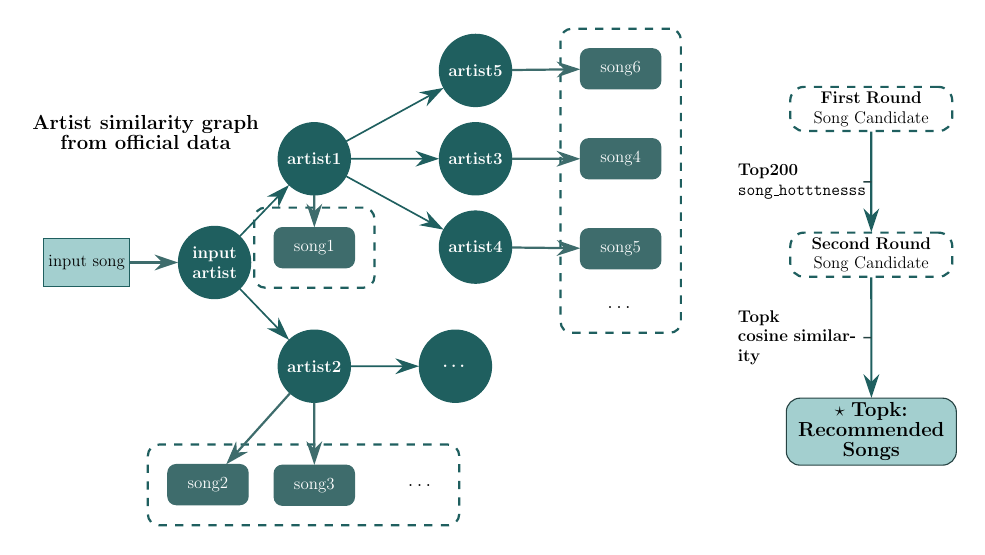
\begin{tikzpicture}[
    scale=0.51, transform shape, 
    node distance=0.8cm and 1.2cm,
    every node/.style={font=\large},
    input/.style={rectangle, draw=aquamarineAccent, fill=aquamarineLight, minimum width=2cm, minimum height=1.2cm, text=black},
    artist/.style={circle, draw=aquamarineAccent, fill=aquamarineAccent, minimum size=1.8cm, text=white, font=\large\bfseries},
    song/.style={rectangle, rounded corners=3pt, draw=aquamarineMid, fill=aquamarineMid, minimum width=2.0cm, minimum height=1.0cm, text=white},
    process/.style={rectangle, rounded corners=5pt, dashed, draw=aquamarineAccent, minimum width=4cm, minimum height=1cm, text width=3.8cm, align=center, text=black},
    final/.style={rectangle, rounded corners=5pt, draw=aquamarineDark, fill=aquamarineLight, minimum width=4cm, minimum height=1cm, text width=4cm, align=center, font=\large\bfseries},
    fitbox/.style={rectangle, rounded corners=4pt, dashed, draw=aquamarineAccent, inner sep=0.25cm},
    arrow_blue/.style={-{Stealth[length=3mm, width=2mm]}, thick, draw=aquamarineMid},
    arrow_red/.style={-{Stealth[length=3mm, width=2mm]}, semithick, draw=aquamarineAccent},
    arrow_purple/.style={-{Stealth[length=3mm, width=2mm]}, semithick, draw=aquamarineDark},
]

% ====== LEFT & MIDDLE PART: GRAPH ======
\node[input] (in_song) {input song};
\node[artist, right=of in_song, align=center] (in_artist) {input \\ artist};
\node[artist, above right=of in_artist, yshift=0.5cm] (artist1) {artist \\ 1};
\node[artist, below right=of in_artist, yshift=-0.5cm] (artist2) {artist \\ 2};
\node[song, below=of artist1] (song1) {song1};
\node[song, below left=of artist2, xshift=0.2cm, yshift=-1.0cm] (song2) {song2};
\node[song, below=of artist2, xshift=0.0cm,yshift=-0.75cm] (song3) {song3};
\node[artist, right=of artist1, xshift=1cm] (artist3) {artist \\ 3};
\node[artist, right=of artist1, xshift=1cm, yshift=-2.2cm] (artist4) {artist \\ 4};
\node[artist, right=of artist1, xshift=1cm, yshift=2.2cm] (artist5) {artist \\ 5};
\node[artist, right=of artist2, xshift=0.5cm] (artist_dots) {\dots};

\node[song, right=of artist3, xshift=0.5cm] (song4) {song4};
\node[song, below=of song4, node distance=4.0cm, yshift=-0.425cm] (song5) {song5};
\node[song, above=of song4, node distance=4.0cm, yshift=0.425cm] (song6) {song6};

% ellipses
\node[below=of song5, node distance=0.7cm, font=\Large] (song_dots_more) {\dots};
\node[right=of song3, node distance=0.7cm, font=\Large] (song_dots_more_more) {\dots};

% --- fit boxes ---
\node[draw=aquamarineAccent, thick, fitbox, fit=(song1)] (fit_s1) {};
\node[draw=aquamarineAccent, thick, fitbox, fit=(song2) (song3) (song_dots_more_more)] (fit_s23) {};
\node[draw=aquamarineAccent, thick, fitbox, fit=(song6) (song4) (song5) (song_dots_more)] (fit_s45) {};

% --- arrows left/middle ---
\draw[arrow_blue] (in_song) -- (in_artist);
\draw[arrow_red] (in_artist) -- (artist1);
\draw[arrow_red] (artist1) -- (artist5);
\draw[arrow_red] (in_artist) -- (artist2);
\draw[arrow_red] (artist1) -- (artist3);
\draw[arrow_red] (artist1) -- (artist4);
\draw[arrow_red] (artist2) -- (artist_dots);

\draw[arrow_blue] (artist1) -- (song1); 
\draw[arrow_blue] (artist2) -- (song2);
\draw[arrow_blue] (artist2) -- (song3);
\draw[arrow_blue] (artist5) -- (song6);
\draw[arrow_blue] (artist3) -- (song4);
\draw[arrow_blue] (artist4) -- (song5);

\node[above=0.2cm of artist1, xshift=-4.2cm, yshift=-1.0cm, align=center] {\Large\textbf{Artist similarity graph} \\ \Large\textbf{from official data}};

% ====== RIGHT PART: PROCESS FLOW ======
\node[draw=aquamarineAccent, thick, process, text=black, right=of song6, xshift=2cm, yshift=-1.0cm] (round1) {\textbf{First Round} \\ Song Candidate};
\node[draw=aquamarineAccent, thick, process, dashed, text=black, below=2.5cm of round1] (round2) {\textbf{Second Round} \\ Song Candidate};
\node[final, below=3.0cm of round2] (topk) {\Large \(\star\) Topk: \\ Recommended Songs};

% arrows right
\draw[arrow_red, thick] (round1) -- (round2);
\draw[arrow_red, thick] (round2) -- (topk);

% midpoints and labels
\coordinate (mid1) at ($(round1.south)!0.5!(round2.north)$);
\coordinate (mid2) at ($(round2.south)!0.5!(topk.north)$);

\node[left=0.2cm of mid1, text width=3cm, align=left] (label_hot) {\textbf{\textbf{Top200} \texttt{song\_hotttnesss}}};
\draw[semithick, draw=aquamarineDark] (label_hot.east) -- (mid1);

\node[left=0.2cm of mid2, text width=3cm, align=left] (label_cos) {\textbf{Topk \\ cosine similarity}};
\draw[semithick, draw=aquamarineDark] (label_cos.east) -- (mid2);

\end{tikzpicture}
    \end{figure}
    \end{frame}

    \begin{frame}{Recommendation Results}
        
        \begin{minipage}[b]{0.5\linewidth}
        \textbf{Input Song:}\\
        \texttt{Song name: Old Man Muse} \\
        \texttt{Artist: Bristols} \\
        \texttt{Track ID: TRMUOZE12903CDF721}
        \end{minipage}%
        \begin{minipage}[b]{0.5\linewidth}
        \textbf{Rank1: } \\
        \texttt{     Song name: Time is due} \\
        \texttt{     Artist: Nine Days Wonder} \\
        \texttt{     Track ID: TRAAQTF128F14ABC48} \\
        \texttt{     Similarity score:} \textbf{0.9518}
        \end{minipage}
        
        \vspace{1.0cm} 
        
        \begin{minipage}[b]{0.5\linewidth}
        \textbf{Rank10: }\\
        \texttt{  Song name: \\ By Morning\_ It's Gone} \\
        \texttt{  Artist: The Deadly Snakes} \\
        \texttt{  Track ID: TRADOCN128EF3542DB} \\
        \texttt{  Similarity score:} \textbf{0.9307}
        \end{minipage}%
        \begin{minipage}[b]{0.5\linewidth}
        \textbf{Rank20: } \\
        \texttt{  Song name: My Baby Left Me} \\
        \texttt{  Artist: Elvis Presley}  \texttt{TRACAGS128F4246062} \\
        \texttt{  Similarity score:} \textbf{0.9163}
        \end{minipage}

    \end{frame}

    \begin{frame}{Comparision between Spark and MapReduce}

    We set up a \textbf{Hadoop cluster} consisting of three nodes, and then implemented the BFS recommendation algorithm both in \textbf{Spark} and \textbf{MapReduce}. 

    \vspace{0.2cm}
    
    Here is the record for their performance:
    
    \vspace{0.3cm}
    
    \begin{minipage}[b]{0.5\linewidth} 
        \textbf{MapReduce Runtime:} \\
        \centering
        \texttt{real    0m18.546s} \\
        \texttt{user    0m26.583s} \\
        \texttt{sys     0m10.735s}
    \end{minipage}%
    \begin{minipage}[b]{0.5\linewidth}
        \textbf{PySpark Runtime:}\\
        \centering
        \texttt{real    0m9.744s} \\
        \texttt{user    0m5.301s} \\
        \texttt{sys     0m2.448s} 
    \end{minipage}

    \vspace{0.3cm}
    
    \textbf{Conclusion}:
        \begin{itemize}
            \item Pyspark runs nearly \textbf{twice} as fast as MapReduce.
            \item Our strategy of presorting the data based on \texttt{song\_hotttnesss} indeed reduce massive calculation and \textbf{significantly boost} the runtime.
        \end{itemize}
    \end{frame}
    
    \begin{frame}{IDEA2: Recommendation on Song Similarity Graph}
    
    What is the song similarity graph? 

    \begin{itemize}
        \item An \textbf{unweighted graph} connecting songs with edges based on \textbf{cosine similarity}.
        \item Customized similarity threshold, e.g. 0.95.
        \item Pros1: \textbf{Efficient graph algorithms} such as BFS can be leveraged for similar song recommendations.
        \item Pros2: Recommendations can be based on \textbf{song playlists} rather than a single song as in IDEA1.
        \item Cons1: Building such a graph may be slow.
    \end{itemize}
    
    \end{frame}

    \begin{frame}{Build Song Similarity Graph}

    How to build the song similarity graph?

    \begin{itemize}
        \item Computing the cosine similarity between every pair of songs has a time complexity of $O(n^2)$, which is infeasible for the scale of the MSD dataset. Therefore, we employ the \textbf{LSH} algorithm to reduce the time complexity to $O(n \log n)$ while ensuring \textbf{parallelism}, making the construction of the song similarity graph possible.
        \item Q: PCA and K-Means can also increase the efficiency, why don't use them?
        \item A: These two algorithms yield \textbf{poor performance} since part of the song features have already been \textbf{PCAed} (\texttt{segments\_timbre}).
        \item \texttt{Explained Variance of first 15/100 dims: 0.564}
        \item \texttt{Silhouette score: -0.091} 
    \end{itemize}

    \end{frame}

    \begin{frame}[fragile]{LSH Introduction}
    
        *Locality Sensitive Hashing (LSH):
        \begin{itemize}
            \item A technique that hashes \textbf{similar input items} (like high-dimensional vectors) into the \textbf{same ``buckets"} with \textbf{high probability}, enabling efficient approximate nearest neighbor search.
            \item Pros1: Significantly \textbf{reduces search time complexity} (average: $O(n \log n)$), making large-scale similarity search feasible.
            \item Pros2: Highly amenable to \textbf{parallelism}, speeding up computation.
            \item Cons1: Provides approximate results, potentially missing some true nearest neighbors (lower recall) or including false positives.
        \end{itemize}

\begin{mycodepython}
lsh = BucketedRandomProjectionLSH(inputCol="scaled_features", outputCol="hashes", bucketLength=1.0, numHashTables=3)
\end{mycodepython}
        
    \end{frame}

    \begin{frame}{Song Similarity Graph Building Workflow}
\begin{tikzpicture}[
    scale=0.5,transform shape,
    node distance=0.8cm and 1.8cm,
    orange_box/.style={rectangle, draw, fill=aquamarineMid, text=white, minimum height=1.2cm, minimum width=2cm, font=\sffamily\bfseries},
    green_circle/.style={circle, draw, fill=aquamarineAccent, text=white, minimum size=1.8cm, font=\sffamily\bfseries},
    gray_box/.style={rectangle, rounded corners, draw, fill=aquamarineGrey, text=white, minimum height=0.7cm, minimum width=1.6cm, font=\sffamily\bfseries},
    green_box/.style={rectangle, rounded corners, draw, fill=aquamarineDark, text=white, minimum height=0.7cm, minimum width=1.6cm, font=\sffamily\bfseries},
    my_arrow/.style={-{{Stealth[length=2.5mm, width=2mm]}}, thick},
    label_text/.style={align=center, font=\sffamily}
]

\node[gray_box] (b2) at (0, 0) {bucket};
\node[gray_box, above=0.7cm of b2] (b1) {bucket};
\node[gray_box, below=0.7cm of b2] (b3) {bucket};
\node[gray_box, below=0.7cm of b3] (b4) {bucket};

\node[green_box, right=of b1] (g1) {graph};
\node[green_box, right=of b2] (g2) {graph};
\node[green_box, right=of b3] (g3) {graph};
\node[green_box, right=of b4] (g4) {graph};

\node[green_circle, left=2.5cm of $(b2)!0.5!(b3)$] (lsh) {LSH};
\node[green_circle, right=2.5cm of $(g2)!0.5!(g3)$] (combine) {Combine};

\node[orange_box, left=of lsh] (df) {DataFrame};
\node[orange_box, left=of df] (avro) {Avro};
\node[orange_box, right=of combine] (finalgraph) {Graph};

\draw[my_arrow] (avro) -- (df);
\draw[my_arrow] (df) -- (lsh);
\draw[my_arrow] (combine) -- (finalgraph);

\draw[my_arrow] (b1) -- (g1);
\draw[my_arrow] (b2) -- (g2);
\draw[my_arrow] (b3) -- (g3);
\draw[my_arrow] (b4) -- (g4);

% LSH -> buckets
\coordinate (lsh_fork) at ($(lsh.east) + (0.8, 0)$);
\draw[my_arrow] (lsh.east) -- (lsh_fork); 
\draw[my_arrow] (lsh_fork) |- (b1.west);
\draw[my_arrow] (lsh_fork) |- (b2.west);
\draw[my_arrow] (lsh_fork) |- (b3.west);
\draw[my_arrow] (lsh_fork) |- (b4.west);

\coordinate (combine_fork) at ($(combine.west) - (0.8, 0)$);
\draw[my_arrow] (combine_fork) -- (combine.west); 
\draw[my_arrow] (g1.east) -| (combine_fork);
\draw[my_arrow] (g2.east) -| (combine_fork);
\draw[my_arrow] (g3.east) -| (combine_fork);
\draw[my_arrow] (g4.east) -| (combine_fork);

\node[label_text, above=0.2cm of df, xshift = -1.8cm] {\Large\textbf{select feature columns}};

\node[label_text, align=center, above=1.35cm of g1, xshift = -1.7cm] (conn_label) {\Large\textbf{connect similar songs based} \\ \Large\textbf{on core feature vectors}};
\coordinate (label_branch) at ($(conn_label.south) + (0, -0.2cm)$);
\draw[] (conn_label.south) -- (label_branch);
\draw[my_arrow] (label_branch) -| ($(b1.east)!0.5!(g1.west)$);
\draw[my_arrow] (label_branch) -| ($(b2.east)!0.5!(g2.west)$);

\node[draw=red, dashed, thick, rounded corners,
      inner sep=0.6cm,
      fit=(lsh) (combine) (b1) (b4)] (parallel_box) {};

\node[label_text, below=0.4cm of parallel_box] {\bfseries \Large{Parallelism}};

\end{tikzpicture}

    \end{frame}

    \begin{frame}{Recommendation Workflow}

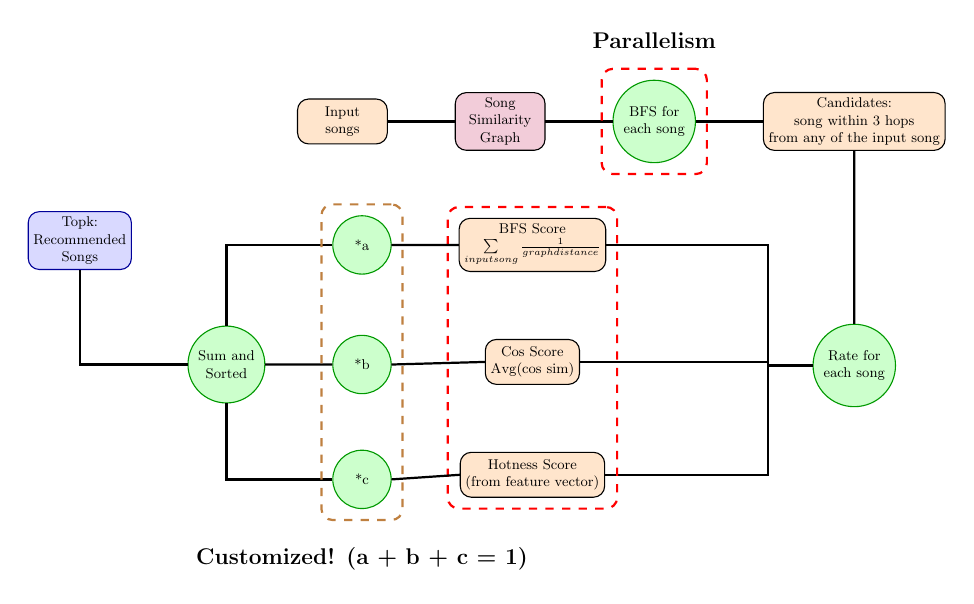
\begin{tikzpicture}[
    scale=0.57, transform shape,
  node distance=1.5cm and 1.5cm,
  every node/.style={font=\small},
  process/.style={rounded corners, draw, minimum width=2cm, minimum height=1cm, align=center},
  greenblock/.style={circle, draw=green!60!black, fill=green!20, minimum size=1.3cm},
  orangeblock/.style={process, fill=orange!20},
  blueblock/.style={process, draw=blue!60!black, fill=blue!15},
  dashedbox/.style={draw=red, dashed, thick, inner sep=4pt, rectangle, rounded corners},
  arrow/.style={thick},
  bend arrow/.style={thick}
]

% Input and Graph
\node[orangeblock] (input) {Input\\songs};
\node[process, fill=purple!20, right=of input] (graph) {Song\\Similarity\\Graph};
\draw[arrow] (input) -- (graph);

% BFS and Candidate
\node[greenblock, right=of graph, align=center] (bfs) {BFS for \\ each song};
\node[orangeblock, right=of bfs] (candidates) {Candidates:\\song within 3 hops\\from any of the input song};
\node[greenblock, below=of candidates, align=center, yshift = -2.36cm] (rate) {Rate for\\each song};

\draw[arrow] (graph) -- (bfs);
\draw[arrow] (bfs) -- (candidates);
\draw[arrow] (candidates) -- (rate);

% Scores
\node[orangeblock, below left=1.5cm and 3.5cm of candidates] (bfs_score) {BFS Score\\$\sum\limits_{\text{input song}} \frac{1}{\text{graph distance}}$};
\node[orangeblock, below=of bfs_score] (cos_score) {Cos Score\\Avg(cos sim)};
\node[orangeblock, below=of cos_score] (hot_score) {Hotness Score\\(from feature vector)};

% From rate to scores (parallel)
\draw[arrow] (rate.west) -- ++(-1.0,0) |- (bfs_score.east);
\draw[arrow] (rate.west) -- ++(-1.0,0) |- (cos_score.east);
\draw[arrow] (rate.west) -- ++(-1.0,0) |- (hot_score.east);

% Red dashed Parallelism box and label
\node[dashedbox, fit=(bfs), label={[yshift=0.3cm,font=\bfseries\Large]Parallelism}] {};
\node[dashedbox, fit=(bfs_score)(cos_score)(hot_score)] {};

% Green weight nodes
\node[greenblock, left=of bfs_score] (wa) {*a};
\node[greenblock, below=of wa, yshift=0.15cm] (wb) {*b};
\node[greenblock, below=of wb, yshift=0.255cm] (wc) {*c};

\draw[arrow] (bfs_score.west) -- (wa.east);
\draw[arrow] (cos_score.west) -- (wb.east);
\draw[arrow] (hot_score.west) -- (wc.east);

% Sum and Sorted
\node[greenblock, left=of wb, align=center] (sum) {Sum and\\Sorted};

\draw[arrow] (wa) -| (sum);
\draw[arrow] (wb) -- (sum);
\draw[arrow] (wc) -| (sum);

% TopK
\node[blueblock, above left=of sum] (topk) {Topk:\\Recommended\\Songs};
\draw[arrow] (sum) -| (topk);

% Customized box
\node[dashedbox, draw=brown, fit=(wa)(wb)(wc), label={[yshift=-8.3cm,font=\bfseries]\Large{Customized! (a + b + c = 1)}}] {};

\end{tikzpicture}

    \end{frame}

    \begin{frame}{Recommendation Results}

    Experiment results on subset \texttt{A.avro}: (\texttt{Runtime: 25.12s})

    \begin{itemize}
        \item $Score = 0.2\times bfs\_score + 0.6 \times cos\_score + 0.2\times hotness\_score$.
        \item The cosine similarity in the figure is computed based on the complete song feature vector.
    \end{itemize}

    \includegraphics[width=\textwidth]{img/Idea2_result.png}
        
    \end{frame}

    \begin{frame}{Remark}

    Features and Advantages:

    \begin{itemize}
        \item \textbf{Fast speed} of searching for recommended songs.
        \item Recommendation on a \textbf{song playlist}.
        \item \textbf{Comprehensive consideration}: the similarity between the recommended song and each song in the playlist, the average similarity across all songs in the playlist, and the hotness of the recommended song.
        \item \textbf{Customized parameters} based on user's preference. For instance, users can increase the parameter for hotness if they want to hear songs that are widely liked within their preferred genres.
    \end{itemize}
        
    \end{frame}
  
    \begin{frame}{IDEA3: Build Fast Indexing in ANN Algorithm}
        HNSW:
        \begin{itemize}
            \item Basics:
                \begin{itemize}
                    \item ``Hierarchical Navigable Small World".
                    \item Pre-built index graph allowing \textbf{high performance similarity search} at $O(\log n)$ complexity.
                    \item Layerly built graph, the higher the layer, the sparser the graph.
                \end{itemize}
            \item Pros:
                \begin{itemize}
                    \item High precision, high recall rate.
                    \item High query speed, no need to reload data.
                \end{itemize}
            \item Cons:
                \begin{itemize}
                    \item Slow index building, memory costing.
                    \item Hard to implement in distributed system.
                \end{itemize}
        \end{itemize}
        LSH:
            \begin{itemize}
                \item Introduced earlier.
            \end{itemize}
    \end{frame}
    \begin{frame}[fragile]{HNSW Pipeline}
    HNSW build and query:
        \begin{mycodepython}
# build index graph
index = faiss.IndexHNSWFlat(TOTAL_DIMS, 64, faiss.METRIC_L2)
for i, file_path in enumerate(part_files):
    df_batch = pd.read_parquet(file_path)
    vectors_list = df_batch["normFeatures"].apply(lambda x: x["values"]).tolist()
    batch_vectors = np.array(vectors_list).astype("float32")
    index.add(batch_vectors)
    for tid, vec in zip(batch_ids, batch_vectors):
        vector_mapping[tid] = vec # store id mappings
faiss.write_index(index, index_file)
# query for ANN results
query_vector_2d = np.array([taste_vector_normalized]).astype("float32")
distances, indices = index.search(query_vector_2d, k + len(input_track_ids))
        \end{mycodepython}
    \end{frame}

    \begin{frame}[fragile]{LSH Pipeline}
    LSH build and query:
    \begin{mycodepython}
# build LSH model
brp = BucketedRandomProjectionLSH(
    inputCol="normFeatures",
    outputCol="hashes",
    bucketLength=0.1, 
    numHashTables=5,
    )
lsh_model = brp.fit(vectorized_df)    lsh_model.write().overwrite().save(path/to/your/model)
# query for ANN results
results_df = lsh_model.approxNearestNeighbors(
    vectorized_df, query_vector, k + len(input_track_ids)
)
    \end{mycodepython}
    \end{frame}

    \begin{frame}{Approximate Nearest Neighbor Workflow}

\begin{tikzpicture}[
    scale=0.5, transform shape,
    node distance=1.2cm and 1.5cm,
    font=\sffamily 
]

\tikzset{
    box_orange/.style={
        rectangle,
        rounded corners,
        fill=aquamarineMid,
        text=white,
        minimum height=1cm,
        minimum width=2.5cm,
        text centered
    },
    circle_green/.style={
        circle,
        fill=aquamarineAccent,
        text=white,
        minimum size=1cm
    },
    box_large_orange/.style={
        rectangle,
        rounded corners,
        fill=aquamarineMid,
        text=white,
        minimum height=4cm,
        minimum width=3.5cm,
        text centered,
        text width=3.5cm
    },
    process_ellipse/.style={
        ellipse,
        fill=aquamarineLight,
        minimum height=2cm,
        minimum width=4cm,
        text centered,
        text width=3.5cm
    },
    box_purple/.style={
        rectangle,
        rounded corners,
        fill=aquamarineDark,
        text=white,
        minimum height=1cm,
        minimum width=2.5cm
    },
    box_grey/.style={
        rectangle,
        fill=aquamarineGrey,
        text=white,
        minimum height=2.2cm,
        minimum width=4.5cm,
        text centered,
        text width=4cm
    },
    box_dashed/.style={
        rectangle,
        rounded corners,
        draw=aquamarineMid,
        text=aquamarineAccent,
        thick,
        dashed,
        minimum height=1cm,
        minimum width=5cm,
        text centered
    },
    arrow_blue/.style={
        -{Stealth[length=3mm, width=2.5mm]},
        thick,
        draw=aquamarineMid
    },
    arrow_red/.style={
        -{Stealth[length=3mm, width=2.5mm]},
        thick,
        draw=aquamarineAccent
    }

}

\node[box_orange] (song1_top) {\Large\textbf{Song1}};
\node[box_orange, below=0.5cm of song1_top] (song2) {\Large\textbf{Song2}};
\node[box_orange, below=0.5cm of song2] (song1_bottom) {\Large\textbf{Song3}};

\node[circle_green, right=1.6cm of song1_top, yshift=0.5cm] (w1) {w1};
\node[circle_green, right=1.6cm of song2, yshift=0.5cm] (w2) {w2};
\node[circle_green, right=1.6cm of song1_bottom, yshift=0.5cm] (w3) {w3};

\node[box_large_orange, right=4.6cm of song2] (avg_vec) {\Large\textbf{Average} \\ \Large\textbf{Feature} \\ \Large\textbf{Vector}};

\node[box_grey, right=2.5cm of avg_vec] (hnsw) {\Large\textbf{HNSW Prebuild Index book}};
\node[box_grey, above=0.2cm of hnsw] (lsh) {\Large\textbf{Spark LSH model catalog}};

\node[box_dashed, below=2cm of hnsw, xshift=3.5cm, yshift=-4.0cm] (reco) {$\star$ \Large\textbf{Topk: Recommended Songs}};

\node[box_purple, below=2.5cm of song1_bottom] (avro) {\Large\textbf{Avro}};
\node[process_ellipse, right=2.58cm of avro] (feature_eng) {\Large\textbf{Feature \\ Engineering into vectors}};
\node[process_ellipse, right=2.58cm of feature_eng] (parquet) {\Large\textbf{Save to Parquet}};

\foreach \source in {song1_top, song2, song1_bottom}
    \draw[arrow_blue] (\source.east) -- (avg_vec.west |- \source);

\draw[arrow_blue] (avg_vec.east) -- (hnsw.west);

\draw[arrow_blue] (hnsw.east) -| (reco.north) node[midway, right, text=black, align=left, xshift=0.3cm, yshift=-3.3cm] {\Large\textbf{cosine} \\ \Large\textbf{similarity}};

\draw[arrow_blue] (avro.east) -- (feature_eng.west);
\draw[arrow_blue] (feature_eng.east) -- (parquet.west);
\draw[arrow_blue] (parquet.north) -- (hnsw.south) node[midway, left, text=black, align=left, xshift=0.0cm, yshift=0.0cm] {\Large\textbf{Faiss HNSW} \\ \Large\textbf{PySpark LSH}};

% \draw[arrow_red] (avro.north) .. controls +(90:3.5cm) and +(180:2.5cm) .. (lsh.west);

\draw[arrow_red] 
  (avro.north) -- ++(0,1) -- ++(-1.5,0) -- ++(0,8) -- ++ (15.9,0) -- (lsh.north);
\end{tikzpicture}

    \end{frame}

    \begin{frame}[fragile]{HNSW recommendation results}
    \begin{minipage}[b]{0.5\linewidth}
        \textbf{HNSW Index Building Runtime:} \\
        \centering
        \texttt{real    0m48.681s} \\
        \texttt{user    11m15.226s} \\
        \texttt{sys     0m11.628s}
    \end{minipage}%
    \begin{minipage}[b]{0.5\linewidth}
        \textbf{HNSW Query Runtime:} \\
        \centering
        \texttt{real    0m1.850s} \\
        \texttt{user    0m4.288s} \\
        \texttt{sys     0m0.522s}
    \end{minipage}
    \vspace{0.2cm}

    \begin{minipage}[b]{0.5\linewidth}
        \vspace{1.0cm}
        \begin{bashcode}
-t "TRMMMYQ128F932D901:0.6"
-t "TRMMMWA128F426B589:0.2"
-t "TRMMMRX128F93187D9:0.2"
        \end{bashcode}
    \end{minipage}%
    \begin{minipage}[b]{0.5\linewidth}
        \centering
        \texttt{
    - Rank 100: \\
    Track ID: TRWWCIE128F1474B69\\
    Title: So Easy Lovin' You \\
    Artist: Ronan Keating \\
    Similarity Score: 0.9974}
    \end{minipage}
    \end{frame}

\begin{frame}[fragile]{LSH recommendation results}
    \begin{minipage}[b]{0.5\linewidth}
        \textbf{LSH Index Building Runtime:} \\
        \centering
        \texttt{real    0m20.144s} \\
        \texttt{user    2m51.856s} \\
        \texttt{sys     0m8.898s}
    \end{minipage}%
    \begin{minipage}[b]{0.5\linewidth}\\
        \textbf{LSH Query Runtime:} \\
        \centering
        \texttt{real    0m22.612s} \\
        \texttt{user    2m27.885s} \\
        \texttt{sys     0m5.764s}
    \end{minipage}
    \begin{minipage}[b]{0.5\linewidth}
        \vspace{1.0cm}
        \begin{bashcode}
-t "TRMMMYQ128F932D901:0.6" 
-t "TRMMMWA128F426B589:0.2" 
-t "TRMMMRX128F93187D9:0.2"
        \end{bashcode}
    \end{minipage}%
    \begin{minipage}[b]{0.5\linewidth}
        \centering
        \texttt{
  - Rank 100:\\
    Track ID: TRGSMVF128F429A85A\\
    Title: Julie Goes Out\\
    Artist: Glow\\
    Cosine Similarity: 0.9665}
    \end{minipage}
    \begin{itemize}
        \item HNSW method is \textbf{fast and accurate}, yet take \textbf{long time} to build.
        \item LSH method is \textbf{relatively slow}, yet take \textbf{shorter time} to build.
        \item Both method supports \textbf{customizable recommend} and \textbf{Song List recommendation!}
    \end{itemize}
\end{frame}

\end{section}

\begin{section}{M3: Year prediction}
    \begin{frame}{Motivation}
    \begin{center}
        \textbf{Classification Task} or \textbf{Regression Task}?
    \end{center}
    \textbf{Intuition:}
        \begin{itemize}
            \item \textbf{Timbre features} who reflect the actual content of the song can be considered as a song's \textbf{unique fingerprints}.
            \item Different songs in different periods should have totally different timbre features $\longrightarrow$ \textbf{classification task?}
            \item Songs whose were produced in near year will likely have similar timbre situation $\longrightarrow$ \textbf{regression task with tolerence year?}
        \end{itemize}
    \end{frame}
    \begin{frame}{Classification pre-look}
        \begin{figure}
            \centering
            \includegraphics[width=0.8\linewidth]{img/classification.pdf}
            \caption{classifcation of PCAed data over year period}
            \label{fig_classification}
        \end{figure}
        \begin{center}
        There is no significant division of timbre features over the year period, \textbf{not suitable for classification}.
        \end{center}
    \end{frame}
    \begin{frame}{Regression with Tolerence Year}
    Pipeline:
        \begin{itemize}
            \item Extract the timbre data for each song out of \texttt{.avro} file, transform it into \texttt{numpy array}.
            \item Label each data point by its year.
            \item Split training set and testing set in ratio $9:1$.
            \item Feed it into models (we tested three kinds of models).
            \item Get regression results, and calculate \texttt{rmse}, \texttt{mae}, \texttt{accuracy}. 
        \end{itemize}
    Models:
        \begin{itemize}
            \item Gradient Boost Tree
            \item Linear Regression (ML library)
            \item XGBoost Regression
        \end{itemize}
    \end{frame}
    \begin{frame}[fragile]{Peek of source code}
    \begin{mycodepython}
# Linear regression
lr = LinearRegression(
    featuresCol="features",
    labelCol=LABEL_COL,
    regParam=0.1,
    elasticNetParam=0.0,
)
# Gradient Boost Tree
gbt = GBTRegressor(
    featuresCol="features", labelCol=LABEL_COL, maxIter=100, maxDepth=5, seed=42
    )
# XGBoost
xgb = SparkXGBRegressor(
    features_col="features", label_col=LABEL_COL, n_estimators=100, max_depth=5, seed=42,
    )
    \end{mycodepython}
    \end{frame}

    \begin{frame}{Regression Statistics}
    \begin{figure}
        \centering
        \includegraphics[width=1.0\linewidth]{img/training_time.png}
        \caption{Training time situation}
        \label{fig:training_time}
    \end{figure}
    \end{frame}

    \begin{frame}{Regression Statistics}
    \begin{figure}
        \centering
        \includegraphics[width=1.0\linewidth]{img/error_metrics.png}
        \caption{Error Situation}
        \label{fig:error}
    \end{figure}
    \end{frame}

    \begin{frame}{Regression Statistics}
    \begin{figure}
        \centering
        \includegraphics[width=1.0\linewidth]{img/accuracy_by_model.png}
        \caption{Accuracy}
        \label{fig:accuracy}
    \end{figure}
    \end{frame}

    \begin{frame}{Remark}
        \textbf{What did we learn from the experiment?}
        \begin{itemize}
            \item Timbre features are \textit{continuous} and evolve \textit{gradually} over years.
            \item Yield accurate regression in the tolerance of 10 years, shrink slow over the decrease of tolerance years. 
            \item Regression models handled this fuzziness better, giving smoother and more accurate predictions.
            \item \textbf{Year prediction is better framed as a regression problem.}
        \end{itemize}
    \end{frame}
\end{section}

% \section{Bibliography}

% \begin{frame}[allowframebreaks]{References}

%     \printbibliography[heading=none]

% \end{frame}

\thankframe

\end{document}

